\chapter{Resultados e discussões}
\label{chap:resultados}

Com o resultado desse trabalho, a comunidade acadêmica passa a dispor e utilizar um sistema web que facilita o fluxo de mercância. A interface idealizada do sistema foi alcançada em sua maior parte, bem como a disponibilização do código fonte.

O sistema proposto foi totalmente desenvolvido de acordo com seus diagramas e requisitos apresentados na seção \ref{chap:etapas_desenvolvimento}. Buscou-se fazer um sistema bonito, intuitivo e robusto para que \textit{queries} ao banco de dados fossem pouco custosas para que o servidor não ficasse sobrecarregado devido as consultadas simultâneas dos usuários.

Divulgado para o público no dia 13 de janeiro de 2020 por meio de redes sociais, o sistema foi calorosamente acolhido pelas pessoas que compõem o âmbito universitário. O link de acesso para o trabalho desenvolvido é \url{http://www.mercadouniversitario.com}, onde será possível realizar o cadastro público para ter acesso aos produtos comercializados, bem como criar uma conta de vendedor para assim divulgar algum produto ao qual deseja-se vender ou comprar.

\section{Comparação entre mockup e resultado obtido}

A telas do sistema serão aqui apresentadas fazendo um comparativo entre o mockup proposto e o resultado alcançado para que seja feita uma melhor análise. As figuras A corresponderão as telas de mockup, já as figuras B serão as mesmas telas alcançadas como resultado. A maior diferença entre o mockup e o resultado gerado foi a escolha da cor principal do sistema, inicialmente foi pensado em um tom roxo, porém, posteriormente foi preferível alterar a cor para um tom de vermelho devido a pesquisas na área de psicologia das cores definir essa cor como estimulante para o consumo de alimentos(espera-se que a maioria dos produtos cadastrados será do gênero alimentício).

As figuras \ref{fig:mockup_login} e \ref{fig:real_login} fazem um comparativo entre a tela de login da aplicação, praticamente não houve mudanças. As figuras \ref{fig:mockup_produtos} e \ref{fig:real_produtos} referenciam a seção de listagem de produtos do sistema, a diferença entre ambos foi básica, foi alterado apenas o botão de busca e campo da palavra-chave para pesquisa. O acesso a um produto foi especificado nas figuras \ref{fig:mockup_produto} e \ref{fig:real_produto}, o campo para definir a quantidade da compra não foi alcançado em relação ao proposto. Observando as figuras \ref{fig:mockup_vendedor} e \ref{fig:real_vendedor} referentes a página do vendedor nota-se a inclusão de duas informações que não foram contempladas no mockup, informações essas que só foram observadas como necessidade do sistema no ato do seu desenvolvimento. A página de pedidos teve poucas alterações como pode ser observado pelas figuras \ref{fig:mockup_pedidos} e \ref{fig:real_pedidos}, foi incluído um botão para cancelar o pedido.

\begin{figure}[htbp!]
  \centering
  \caption{(A) Tela de login proposta}
  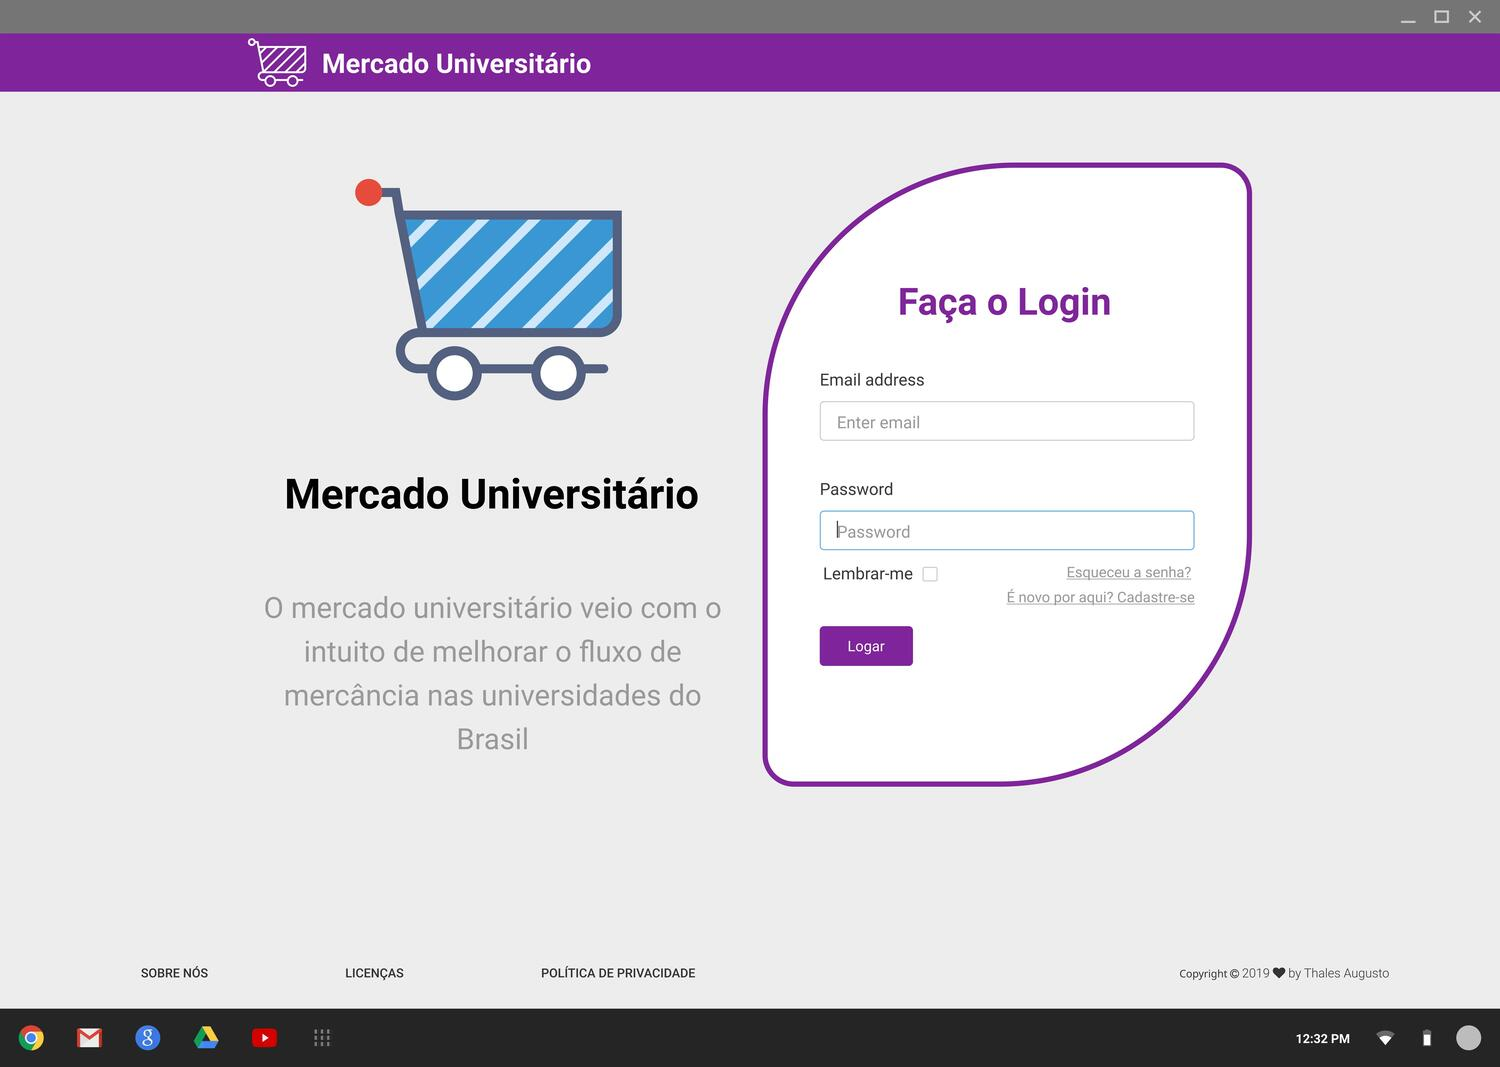
\includegraphics[width=1\textwidth]{figs/mockup/login.jpg}
    \legend{Fonte: Elaborada pelo autor.}
    \label{fig:mockup_login}
\end{figure}

\begin{figure}[htbp!]
  \centering
  \caption{(B) Tela de login obtida como resultado}
  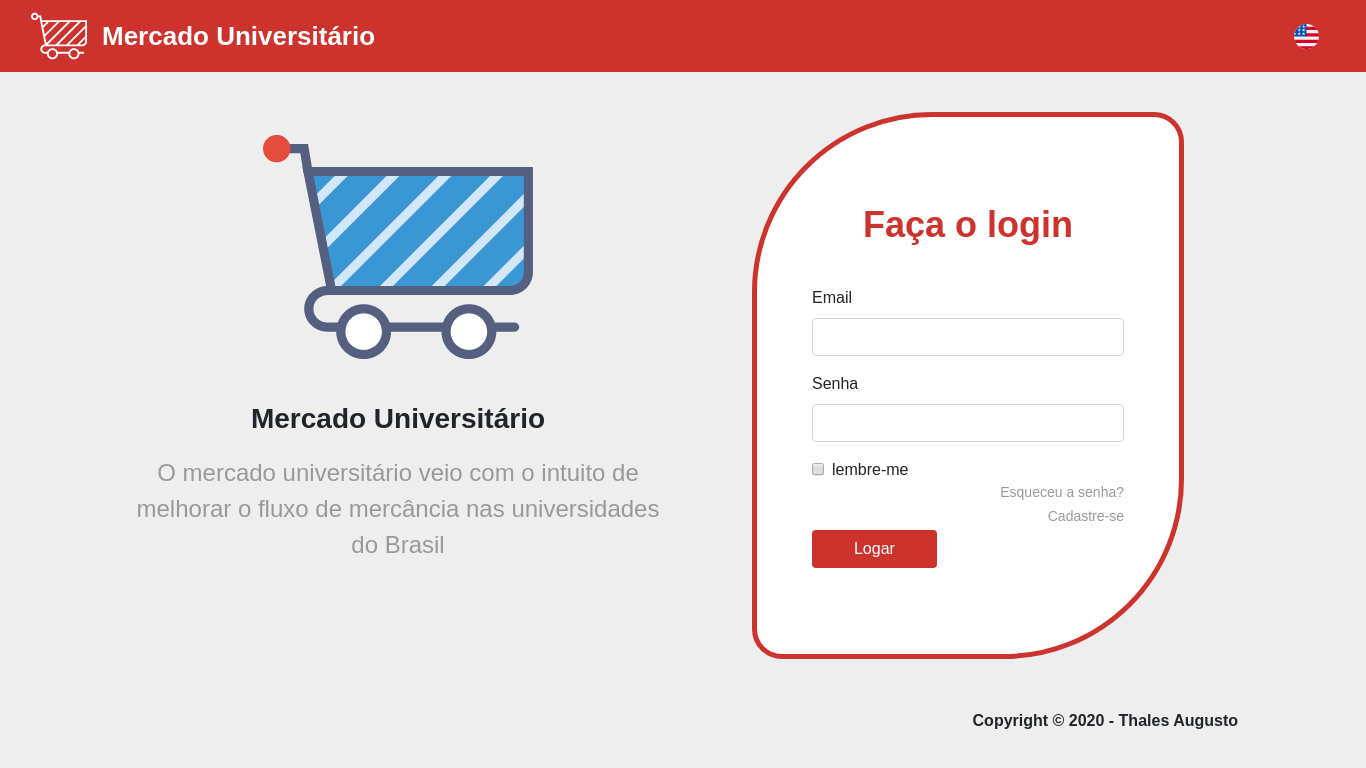
\includegraphics[width=1\textwidth]{figs/resultado/login.png}
    \legend{Fonte: Elaborada pelo autor.}
    \label{fig:real_login}
\end{figure}

\begin{figure}[htbp!]
  \centering
  \caption{(A) Tela de produtos proposta}
  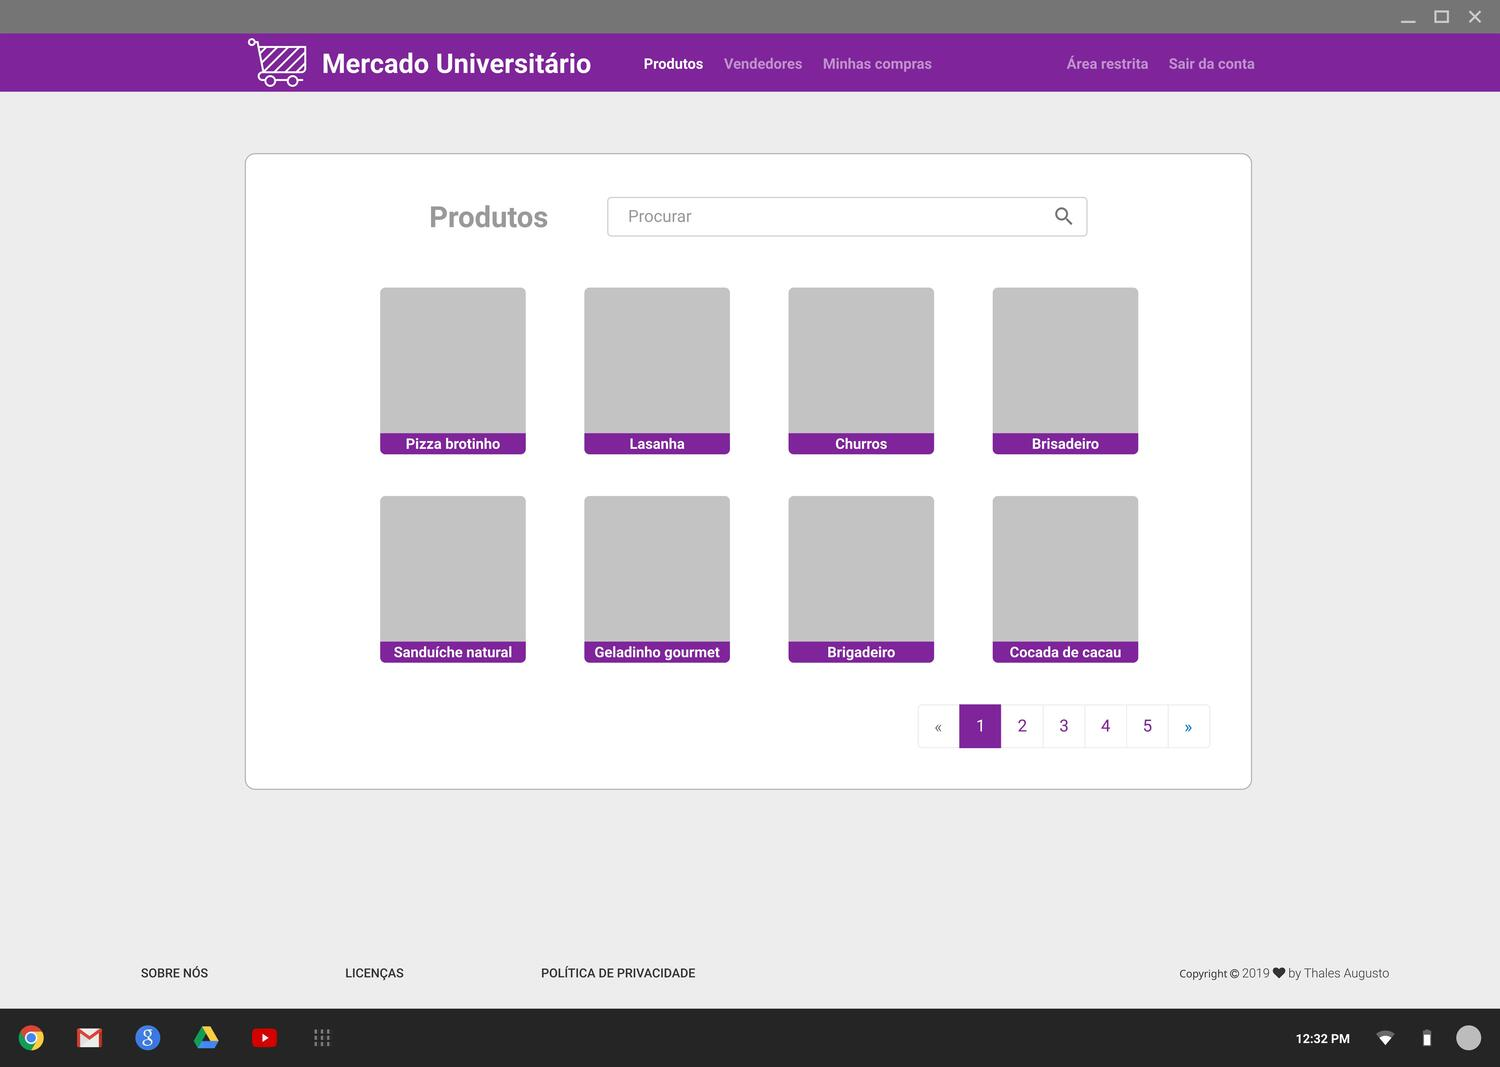
\includegraphics[width=1\textwidth]{figs/mockup/produtos.jpg}
    \legend{Fonte: Elaborada pelo autor.}
    \label{fig:mockup_produtos}
\end{figure}

\begin{figure}[htbp!]
  \centering
  \caption{(B) Tela de produtos obtida como resultado}
  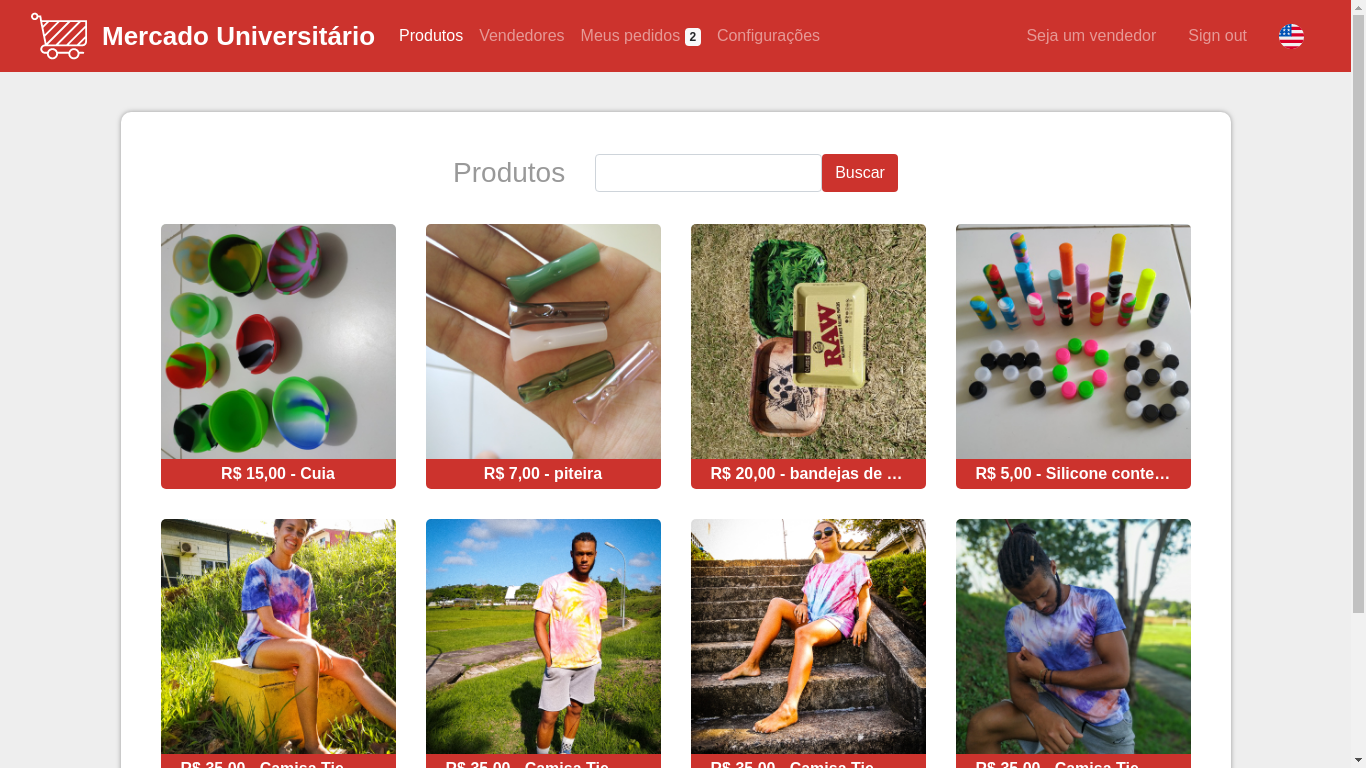
\includegraphics[width=1\textwidth]{figs/resultado/produtos.png}
    \legend{Fonte: Elaborada pelo autor.}
    \label{fig:real_produtos}
\end{figure}

\begin{figure}[htbp!]
  \centering
  \caption{(A) Tela individual de produto proposta}
  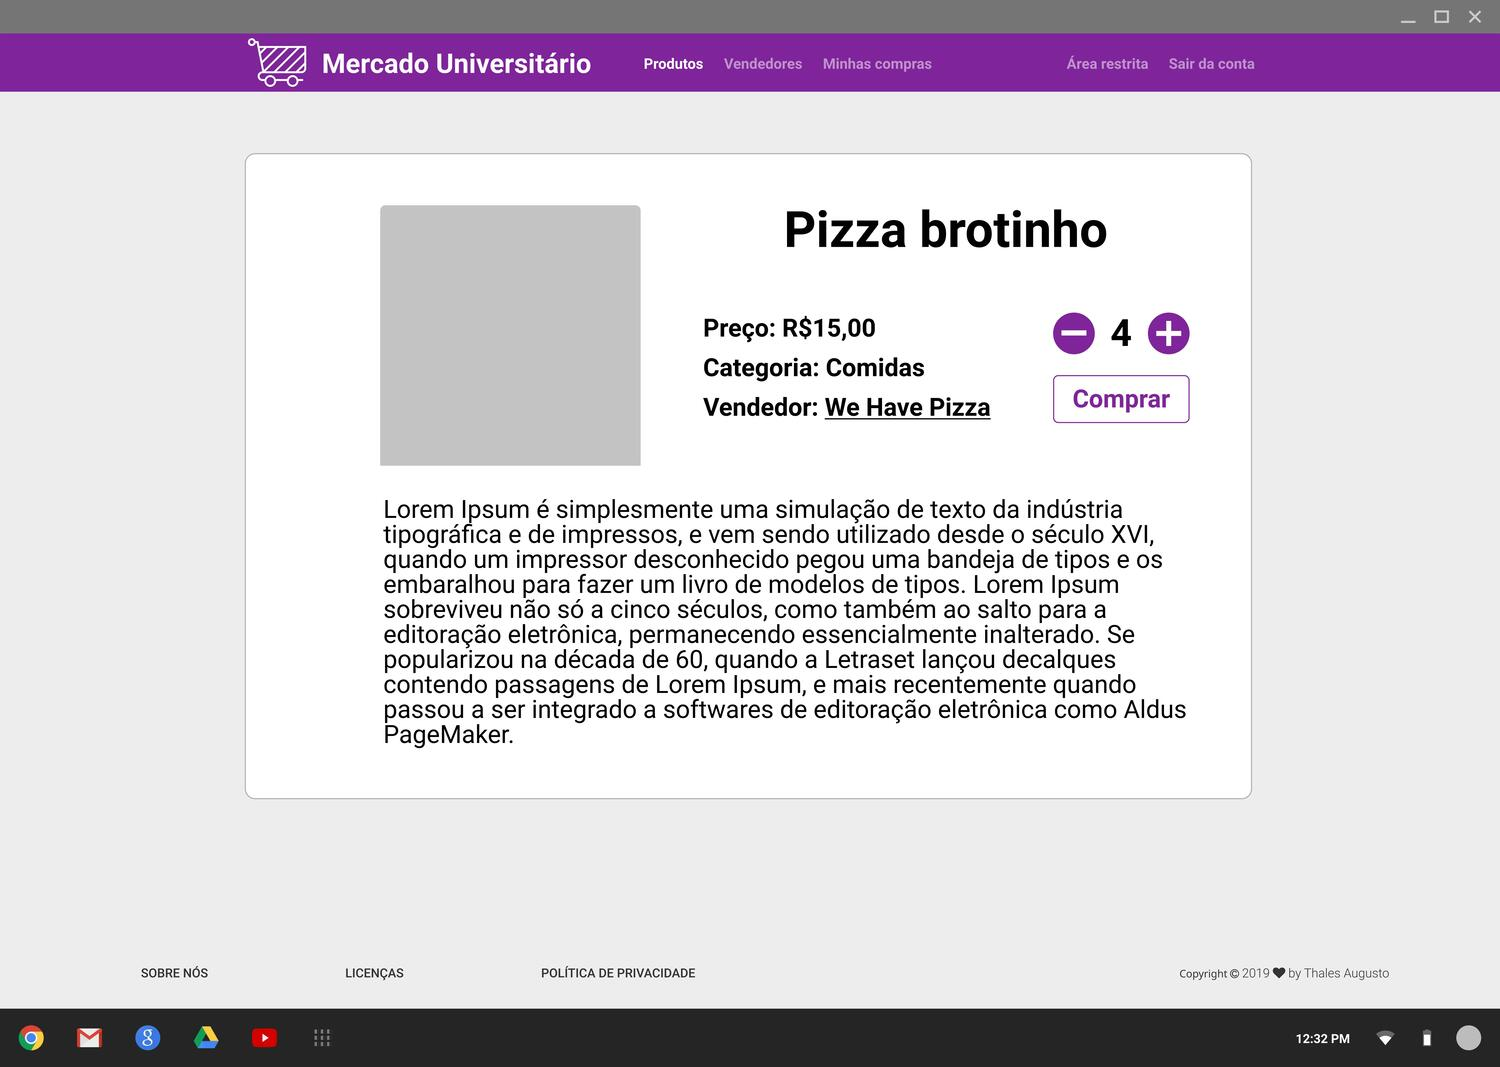
\includegraphics[width=1\textwidth]{figs/mockup/produto.jpg}
    \legend{Fonte: Elaborada pelo autor.}
    \label{fig:mockup_produto}
\end{figure}

\begin{figure}[htbp!]
  \centering
  \caption{(B) Tela individual de produto obtida como resultado}
  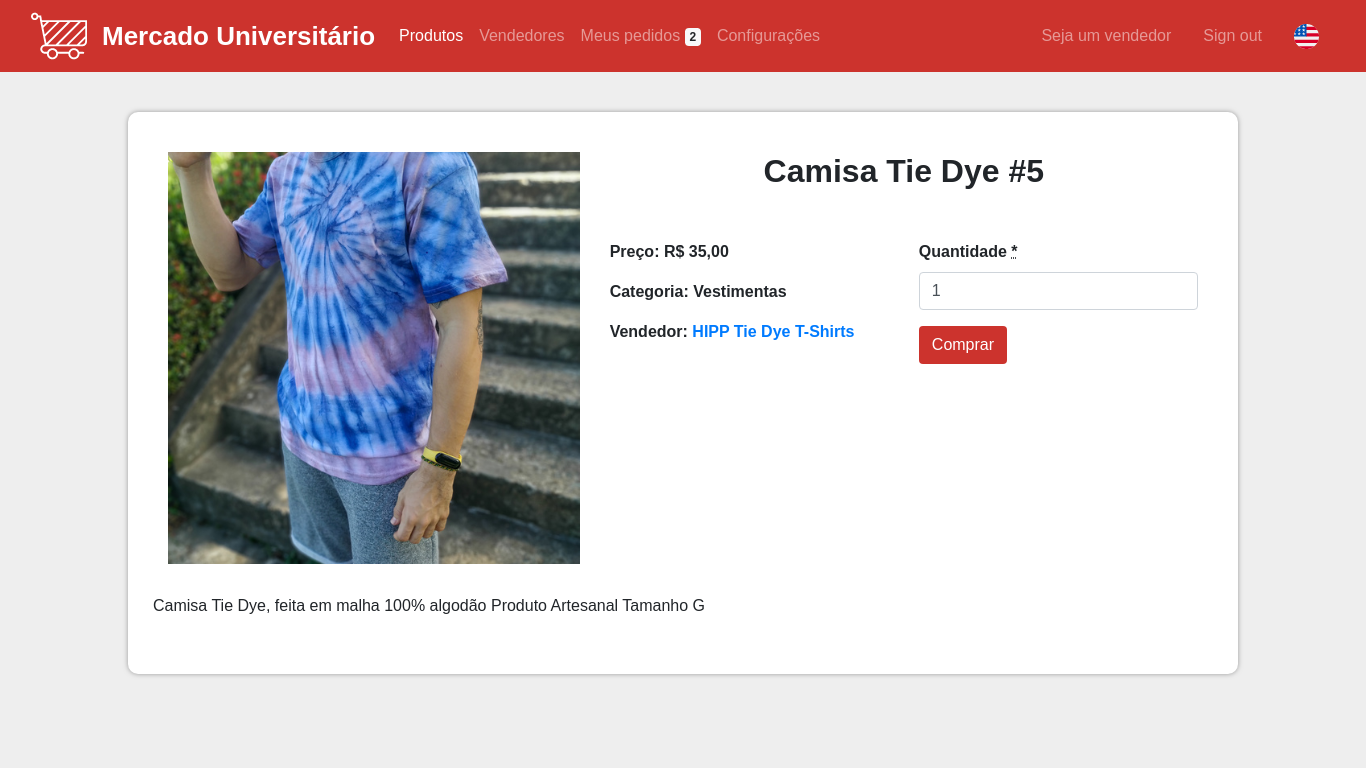
\includegraphics[width=1\textwidth]{figs/resultado/produto.png}
    \legend{Fonte: Elaborada pelo autor.}
    \label{fig:real_produto}
\end{figure}

\begin{figure}[htbp!]
  \centering
  \caption{(A) Tela individual do vendedor proposta}
  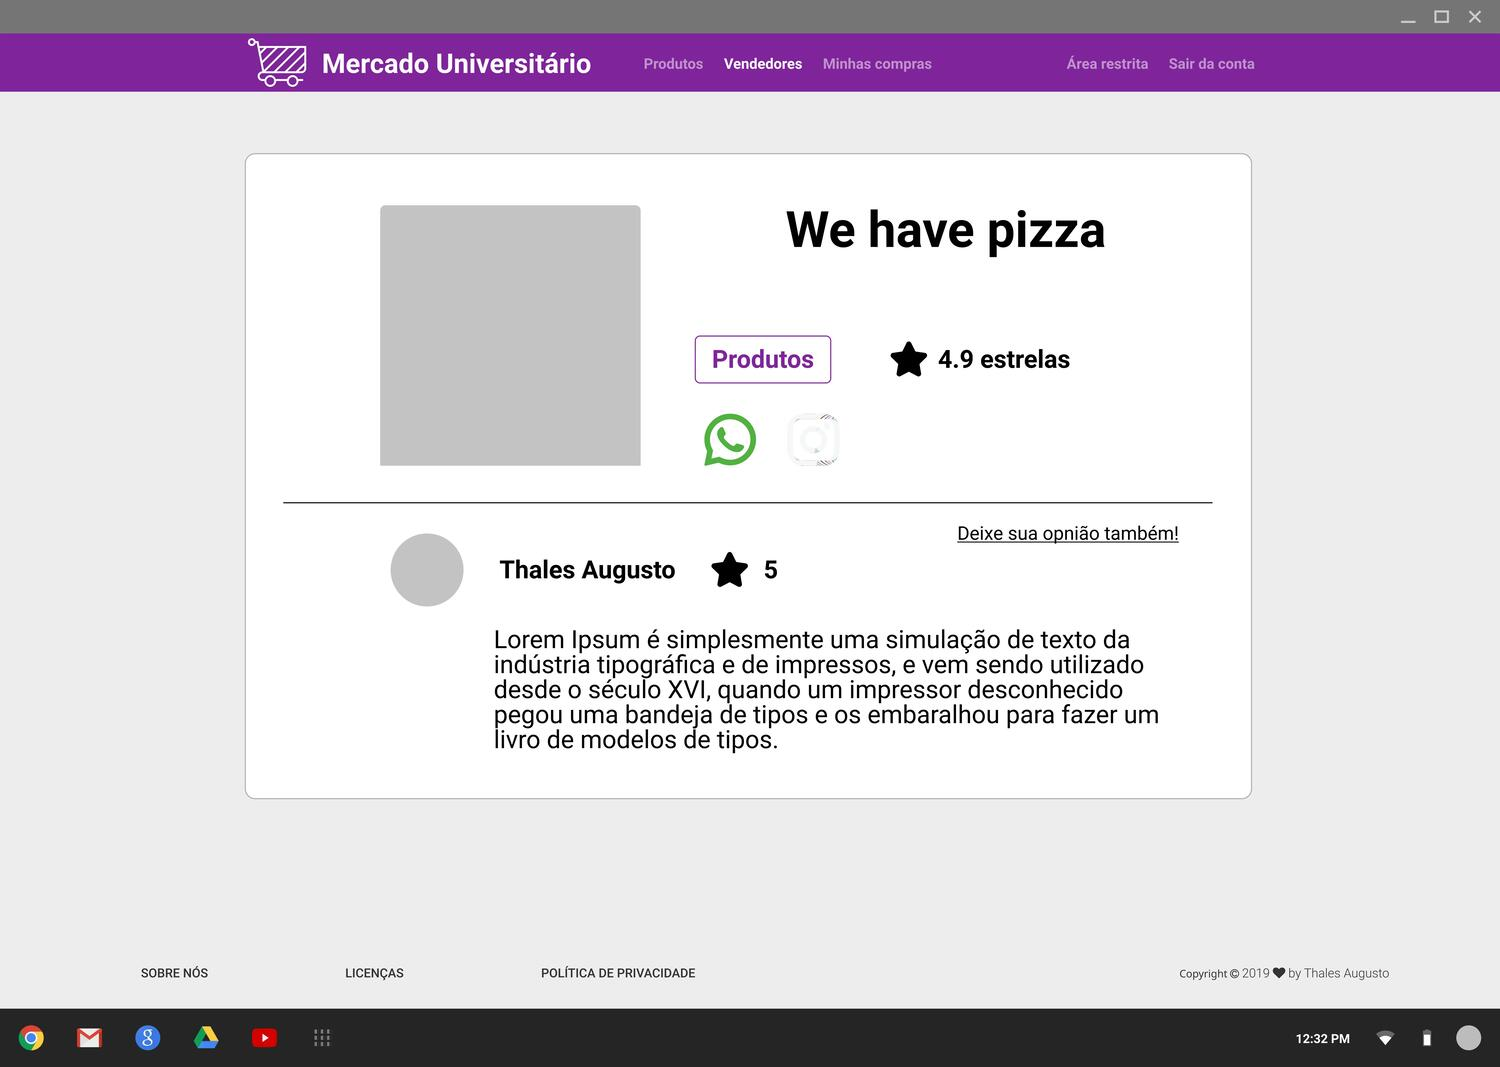
\includegraphics[width=1\textwidth]{figs/mockup/vendedor.jpg}
    \legend{Fonte: Elaborada pelo autor.}
    \label{fig:mockup_vendedor}
\end{figure}

\begin{figure}[htbp!]
  \centering
  \caption{(B) Tela individual do vendedor obtida como resultado}
  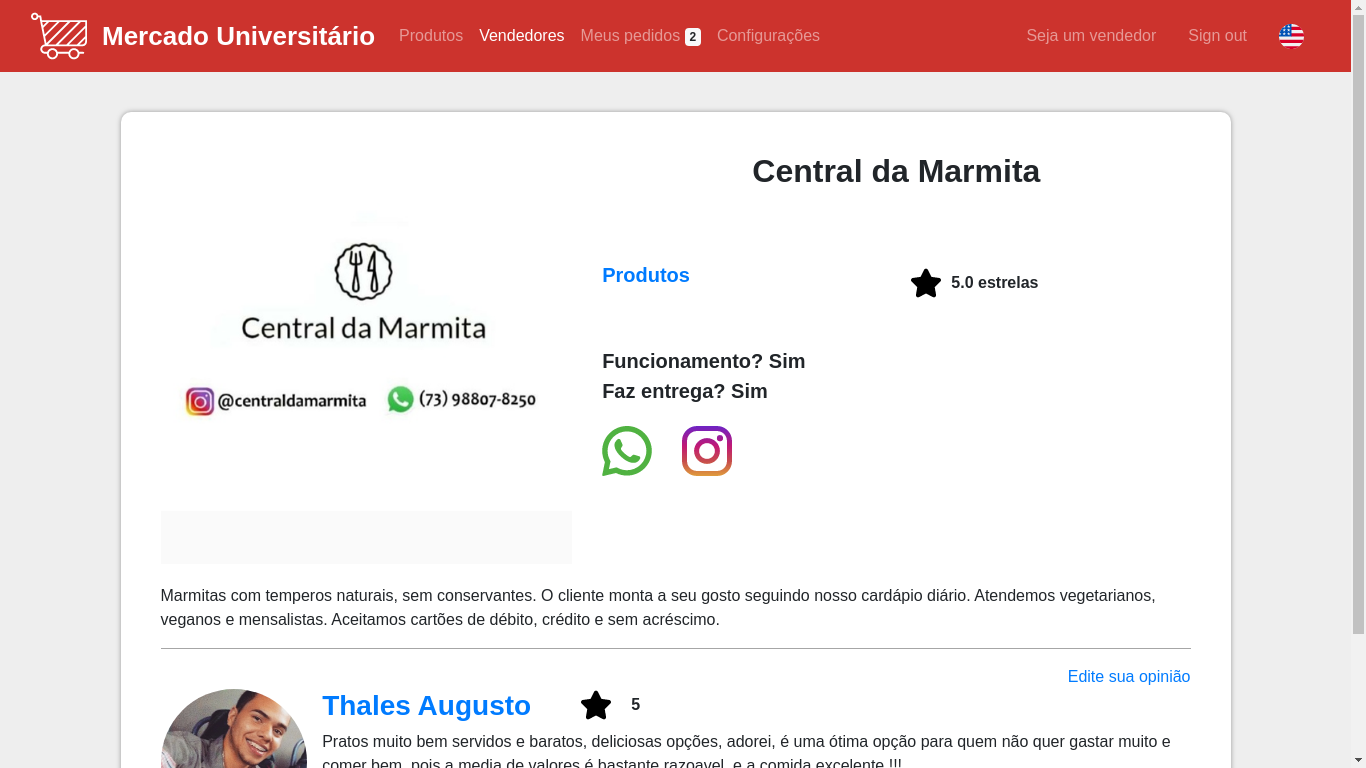
\includegraphics[width=1\textwidth]{figs/resultado/vendedor.png}
    \legend{Fonte: Elaborada pelo autor.}
    \label{fig:real_vendedor}
\end{figure}

\begin{figure}[htbp!]
  \centering
  \caption{(A) Tela de pedidos proposta}
  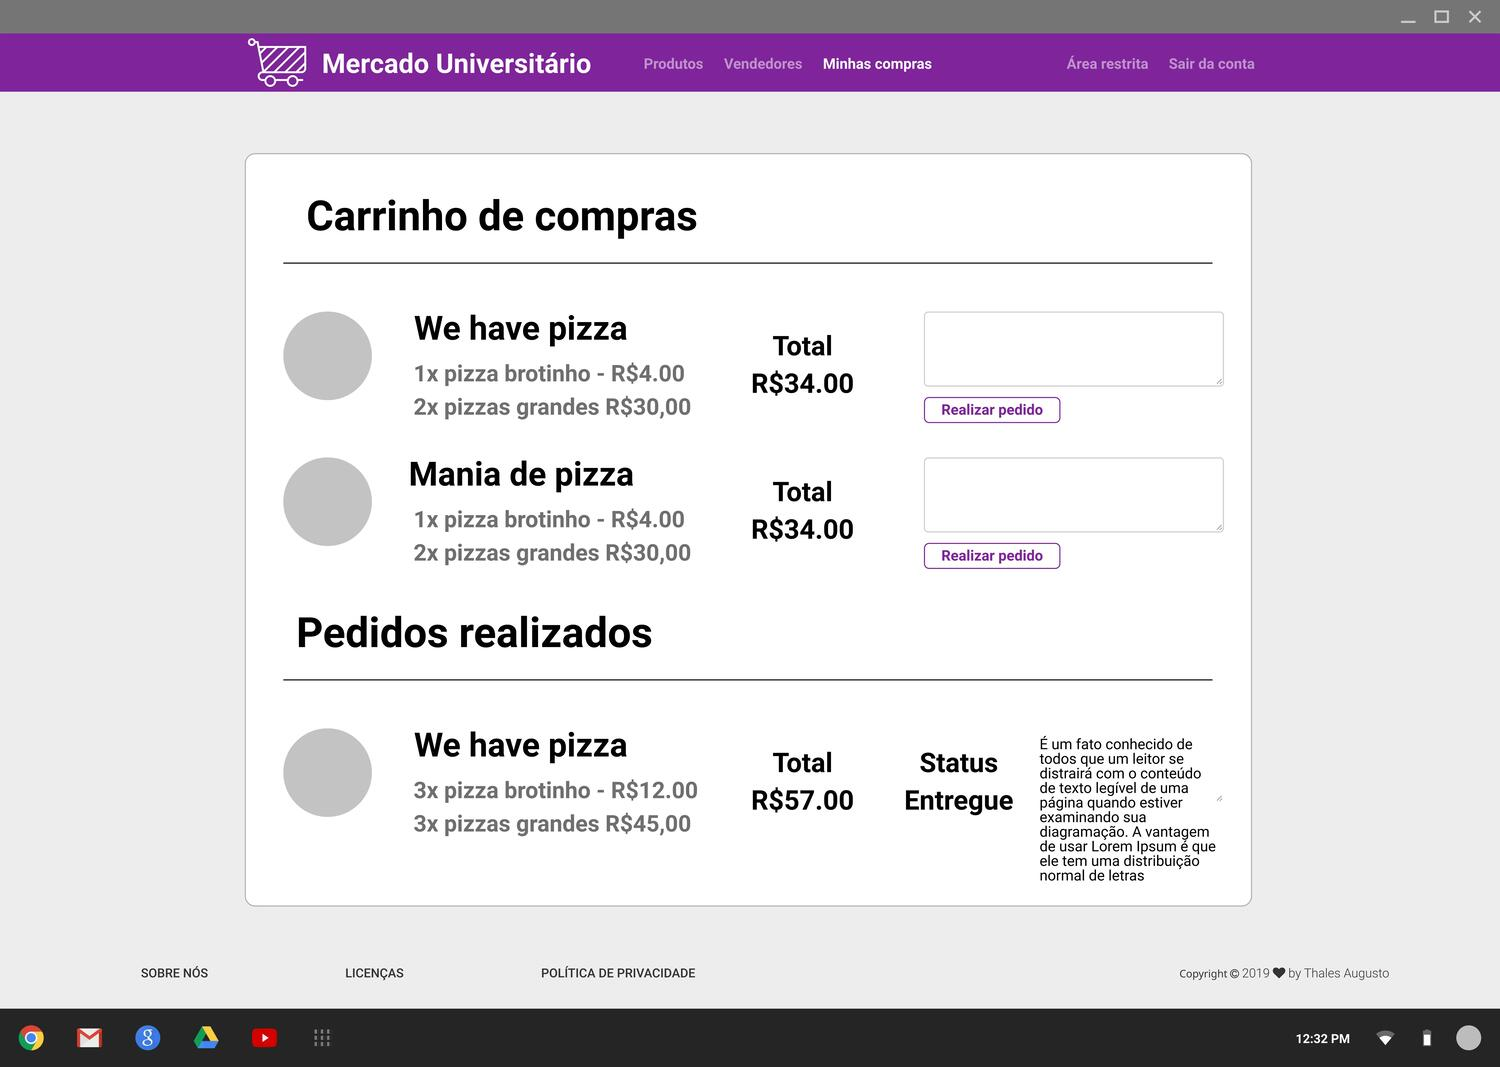
\includegraphics[width=1\textwidth]{figs/mockup/carrinho.jpg}
    \legend{Fonte: Elaborada pelo autor.}
    \label{fig:mockup_pedidos}
\end{figure}

\begin{figure}[htbp!]
  \centering
  \caption{(B) Tela de pedidos obtida como resultado}
  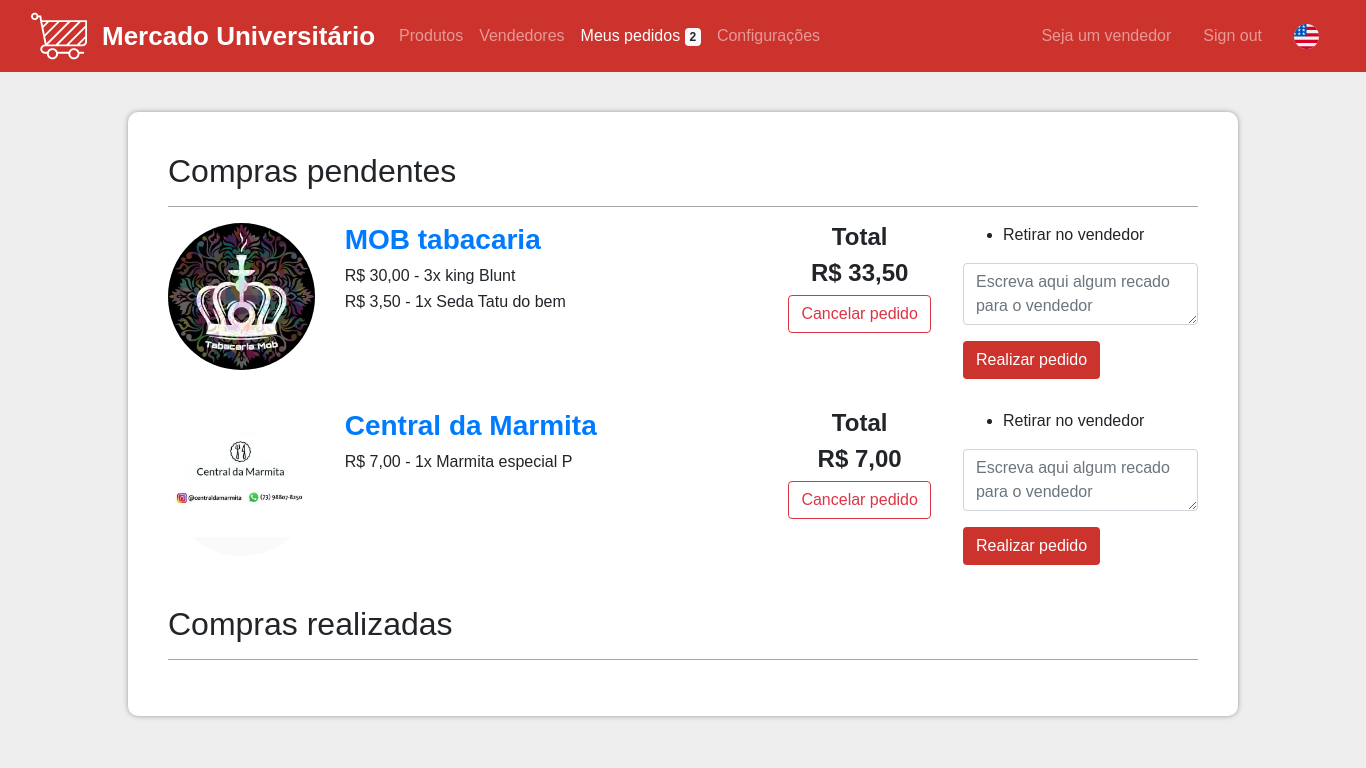
\includegraphics[width=1\textwidth]{figs/resultado/carrinho.png}
    \legend{Fonte: Elaborada pelo autor.}
    \label{fig:real_pedidos}
\end{figure}

\section{Validação do sistema}

Como citado na seção \ref{section:tdd}, foi utilizado a metodologia TDD para desenvolvimento do trabalho, dessa forma foi possível validar o sistema implementado por meio de testes automatizados. A assertividade desses testes serão demonstrados aqui nesta seção e poderá ser confirmada por qualquer pessoa que deseja, pois o código fonte de toda aplicação está disponível no Github por meio do link \url{https://github.com/tarv7/mercado-universitario}.

Foi avaliado de forma sistemática toda a implementação técnica desenvolvida até o momento, buscando-se uma melhor eficiência e qualidade do código da aplicação. Serão realizados quatro tipos de testes automatizados no Mercado Universitário. Testes unitários e integração, testes de segurança e testes de qualidade do código, tais testes serão apresentados a seguir.

\subsection{Testes unitários e integração}
Foi utilizada a gem RSpec para esse tipo de teste. Tal ferramenta foi apresentada na seção \ref{rspec}. De acordo com a figura \ref{fig:rspec} foram realizados 102 exemplos de testes na aplicação, tais testes conseguiram cobrir 92.9\% de todo o código da   aplicação sem que ocorresse nenhuma falha. Tal resultado se mostra bastante satisfatório, uma vez que se aproxima bastante de 100\% de cobertura do código e não apresenta nenhuma falha.
\begin{figure}[htbp!]
  \centering
  \caption{Saída do terminal para teste automatizado unitário e de integração utilizando a \textit{gem} RSpec}
  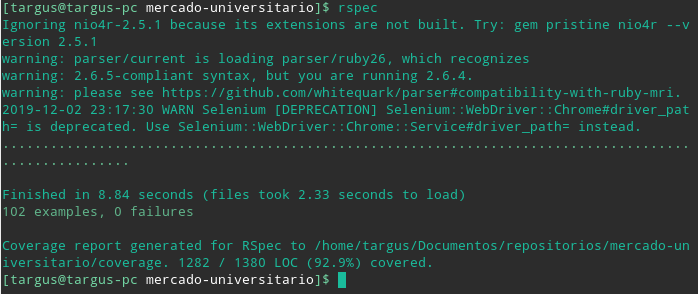
\includegraphics[width=1\textwidth]{figs/rspec.png}
    \legend{Fonte: Elaborada pelo autor.}
    \label{fig:rspec}
\end{figure}
\subsection{Testes de segurança}
Foram utilizadas duas \textit{gems} para realizar esse teste de grande importância para a aplicação. A \textit{gem} Brakeman em conjunto com a \textit{gem} Bundle Audit são suficientes para explorar as principais vulnerabilidades das aplicações web. Como é observado nas imagens \ref{fig:brakeman} e \ref{fig:audit}, não foram encontradas nenhuma vulnerabilidade na aplicação.
\begin{figure}[htbp!]
  \centering
  \caption{Saída do terminal para teste automatizado de segurança utilizando a \textit{gem} Brakeman}
  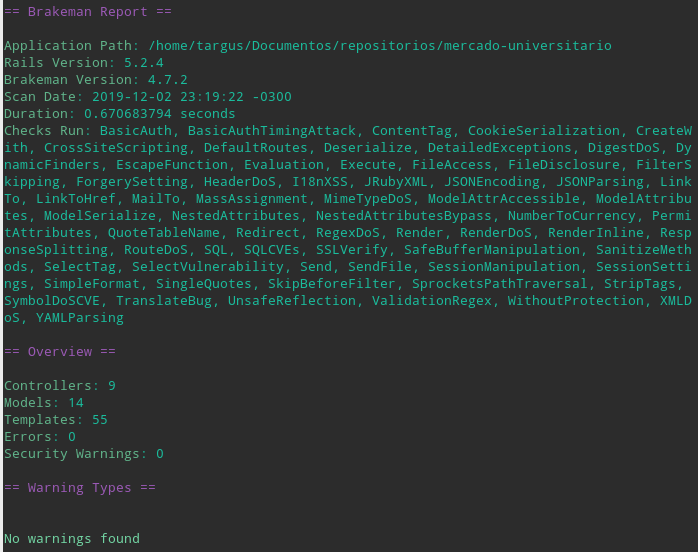
\includegraphics[width=1\textwidth]{figs/brakeman.png}
    \legend{Fonte: Elaborada pelo autor.}
    \label{fig:brakeman}
\end{figure}
\begin{figure}[htbp!]
  \centering
  \caption{Saída do terminal para teste automatizado de segurança utilizando a \textit{gem} Bundle Audit}
  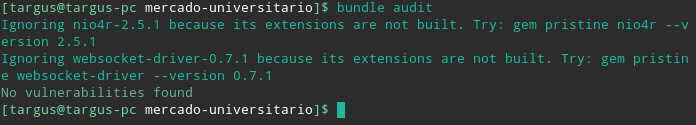
\includegraphics[width=1\textwidth]{figs/bundle_audit.png}
    \legend{Fonte: Elaborada pelo autor.}
    \label{fig:audit}
\end{figure}
\subsection{Testes de qualidade do código}
Para ser possível garantir uma boa manutenção e legibilidade futura do código, foi necessário utilizar a \textit{gem} Rubocop(apresentada na seção \ref{rubocop}). Como observado na figura \ref{fig:rubocop}, foram verificadas as boas práticas de programação determinadas pelo Rails em 71 arquivos do trabalho, não foi encontrada nenhuma ofensa no código.
\begin{figure}[htbp!]
  \centering
  \caption{Saída do terminal para verificação da qualidade do código utilizando a gem Rubocop}
  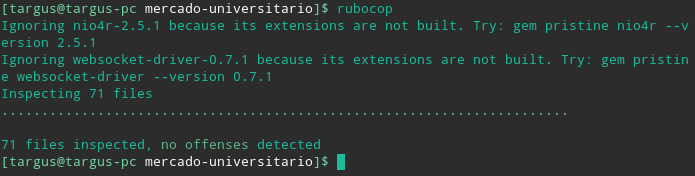
\includegraphics[width=1\textwidth]{figs/rubocop.png}
    \legend{Fonte: Elaborada pelo autor.}
    \label{fig:rubocop}
\end{figure}
